\documentclass[sigconf,nonacm]{acmart}

\setcopyright{none}
\settopmatter{printacmref=false, printccs=false, printfolios=true}
\renewcommand\footnotetextcopyrightpermission[1]{}
\pagestyle{plain}

\usepackage{booktabs}
\usepackage{graphicx}
\usepackage{array}

\graphicspath{{../results/figures/}}

\title{Do LLM Agents Obey Institutions?\\Incentive Reasoning versus Authority Cues in Correlated-Equilibrium Games}

\author{Suyc24}
\affiliation{%
  \institution{Game Theory Course Project}
  \city{}
  \country{}
}
\email{}

\begin{document}

\begin{abstract}
Correlated equilibrium gives a precise game-theoretic account of when private
recommendations from a mediator are self-enforcing. This project asks whether
large language models (LLMs), when prompted as game-playing agents, obey such
recommendations because they reason about incentive compatibility, or because
they respond to institutional authority cues such as a ``trusted mediator'' and
the label ``correlated equilibrium.'' We build a reproducible Python pipeline
covering six normal-form games, four frontier model labels, real and fake
mediator distributions, behavioral choice prompts, analytical prompts, and
two-turn intervention prompts. The main finding is a knowledge--action gap.
Models strongly comply with real correlated-equilibrium recommendations, but
they also comply with fake non-incentive-compatible recommendations when those
recommendations are backed by institutional language. In the original four
games, fake distributions labeled as correlated equilibria receive 0.551 parsed
compliance, compared with 0.320 when the same distributions are shown without
the label. In two harder follow-up games, Rock-Paper-Scissors and a 3x3
dominance game, the same label effect remains visible. However, explicit
auditing prompts can reverse the behavior: in a small DeepSeek-only C7
intervention pilot, checklist-style and skeptical-audit prompts produce zero
compliance with fake recommendations and perfect conditional best-response
choice. These results suggest that LLM agents possess relevant incentive
knowledge, but direct action prompts often make institutional obedience more
salient than mechanism auditing.
\end{abstract}

\maketitle

\section{Introduction}

Institutions often work by turning strategic uncertainty into structured
recommendations. A mediator, protocol, legal rule, platform, or contract can
tell each participant what to do. In classical game theory, correlated
equilibrium (CE) formalizes when such recommendations are self-enforcing:
conditional on receiving one's private recommendation, no player should want to
deviate~\cite{aumann1974subjectivity,aumann1987correlated}. This makes CE a
natural testbed for studying LLM agents. If LLMs are deployed as strategic
participants in mediated systems, a key question is not only whether they know
the definition of CE, but whether they use that knowledge when acting.

This project studies the following question:

\begin{quote}
\emph{Do LLM agents obey institutions because they reason through incentive
compatibility, or because authority cues make obedience salient?}
\end{quote}

The distinction matters. An agent that follows a real CE because obedience is
optimal is behaving in a game-theoretically appropriate way. An agent that also
follows a fake, non-incentive-compatible distribution merely because it is
called a CE is responding to the institution's label rather than to its
incentive structure. The latter behavior is concerning for any setting where an
LLM must audit a rule, protocol, or recommendation rather than simply defer to
it.

We implement a full experimental pipeline for six normal-form games. The first
four are standard 2x2 games: Battle of the Sexes, Chicken, Pure Coordination,
and Prisoner's Dilemma. The two follow-up games are a 3x3 zero-sum
Rock-Paper-Scissors game and a 3x3 game with strictly dominant actions. Each
game contains a real CE distribution and a fake distribution that fails
incentive compatibility. Four model labels are called through a single
OpenAI-compatible endpoint: \texttt{gpt-5.4}, \texttt{claude-opus-4.6},
\texttt{gemini-3.1-pro}, and \texttt{deepseek-v4-pro}. Each model is prompted as
Player 1.

The core design compares behavioral choice prompts with analytical prompts. In
behavioral mode, the model receives a private recommendation and must choose an
action. In analytical mode, the model must compute whether a distribution is a
CE. The crucial contrast is between a fake CE condition where the non-IC
distribution is falsely labeled as a CE and an honest non-CE condition where the
same distribution is shown without the label.

The project makes three contributions:

\begin{enumerate}
  \item It provides a reproducible pipeline for CE compliance experiments,
  including game validation, prompt generation, API execution, parsing,
  best-response annotation, and visualization.
  \item It shows that LLM compliance is not explained by incentive reasoning
  alone: institutional labels and trusted-mediator framing can induce obedience
  to fake recommendations.
  \item It introduces a low-cost C7 intervention pilot showing that explicit
  audit prompts can move an LLM from obedience to conditional best-response
  behavior.
\end{enumerate}

\section{Background}

Nash equilibrium requires that each player's strategy be a best response to the
other players' strategies~\cite{nash1950equilibrium}. Correlated equilibrium
generalizes this idea by allowing a public distribution over joint actions and
private recommendations to the players. A distribution is a CE if, for every
player and every recommendation that occurs with positive probability, the
player's expected payoff from obeying is at least as high as the payoff from
switching to any alternative action, conditional on receiving that
recommendation~\cite{aumann1987correlated,osborne1994course}.

This conditional structure makes CE a useful behavioral probe. If a model sees a
payoff matrix and a mediator distribution, it can in principle compute whether
obedience is rational. But LLMs are also instruction-following systems trained
to be responsive to natural-language cues~\cite{brown2020language,bommasani2021opportunities}.
The words ``trusted mediator'' and ``correlated equilibrium'' may themselves
create pressure toward obedience. The experiment therefore separates three
mechanisms:

\begin{itemize}
  \item \textbf{Incentive reasoning}: the model follows the recommendation
  because obeying maximizes conditional expected payoff.
  \item \textbf{Authority-cue obedience}: the model follows because a trusted
  mediator or CE label makes obedience appear normatively appropriate.
  \item \textbf{Activated auditing}: the model audits the mechanism before
  acting and deviates when the institution is not incentive-compatible.
\end{itemize}

\section{Experimental Design}

\subsection{Games}

The experiment contains six two-player normal-form games. The first four are
small benchmark games:

\begin{itemize}
  \item \textbf{Battle of the Sexes}: a coordination game with conflicting
  preferred equilibria.
  \item \textbf{Chicken}: a Hawk--Dove style game where obedience sometimes
  requires restraint.
  \item \textbf{Pure Coordination}: a coordination game with a Pareto-dominated
  equilibrium.
  \item \textbf{Prisoner's Dilemma}: a dominant-strategy-defection control.
\end{itemize}

The two follow-up games add a larger action space:

\begin{itemize}
  \item \textbf{Rock-Paper-Scissors}: a 3x3 zero-sum cyclic game. The real CE is
  uniform over all nine outcomes. The fake distribution is uniform over the six
  off-diagonal outcomes.
  \item \textbf{3x3 Dominated Strategy}: a game where Down is strictly dominant
  for Player 1 and Right is strictly dominant for Player 2. The real CE is the
  pure outcome (Down, Right). The fake distribution recommends dominated
  actions with positive probability.
\end{itemize}

Every real distribution is checked numerically for incentive compatibility.
Every fake distribution is checked to fail incentive compatibility.

\subsection{Conditions}

Table~\ref{tab:conditions} lists the prompt conditions. The model is always
Player 1 and is told that its payoff is the first number in each payoff cell.

\begin{table}[t]
  \centering
  \caption{Experimental conditions.}
  \label{tab:conditions}
  \begin{tabular}{p{0.18\columnwidth}p{0.72\columnwidth}}
    \toprule
    Condition & Description \\
    \midrule
    C1 & Trusted mediator recommendation; distribution hidden. \\
    C2 & Real CE distribution shown; no CE label. \\
    C3 & Real CE distribution shown and labeled as CE. \\
    C4 & Fake non-IC distribution falsely labeled as CE. \\
    C5 & Same fake distribution shown without the CE label. \\
    C6 & Analytical CE-identification task, real or fake. \\
    C7 & Analytical turn followed by behavioral action. \\
    C7-I & Optional fake-CE interventions: own-audit and skeptical-audit prompts. \\
    \bottomrule
  \end{tabular}
\end{table}

The optional C7 intervention conditions are not part of the default full run.
They were used only in a low-cost DeepSeek-only pilot on the two follow-up
games:

\begin{itemize}
  \item \texttt{C7-fake-own-audit}: audit Player 1's private recommendation
  using an incentive-compatibility checklist.
  \item \texttt{C7-fake-skeptical}: treat the CE label as an unverified
  institutional claim and audit it before acting.
\end{itemize}

\subsection{Models, Sample Size, and Data Handling}

The main dataset uses $N=5$ trials per experimental cell. The final raw log
contains 2757 JSONL records. After filtering to trial numbers $0$--$4$ and
deduplicating repeated attempts by preferring successful, parsed, and complete
records, the analysis contains 1860 records. This count includes the
DeepSeek-only intervention pilot, which has $N=2$ per intervention cell.

The raw files retain API failures and empty responses. The analysis reports both
attempted compliance and parsed compliance where relevant. The paper emphasizes
parsed compliance for behavioral tendency, while also noting timeout and parsing
gaps as limitations.

\subsection{Metrics}

For behavioral prompts, the primary metric is compliance: whether the parsed
first-line action equals the mediator's recommendation. Because fake CE
recommendations are not incentive-compatible, compliance and rational
best-response behavior point in opposite directions for C4 and C5.

The analysis also annotates each behavioral response with:

\begin{itemize}
  \item whether it mentions payoff calculation;
  \item whether it mentions deviation or profitable deviation;
  \item whether it invokes CE language;
  \item whether it invokes mediator trust;
  \item whether it expresses skepticism toward the institutional label;
  \item whether the parsed action equals Player 1's conditional best response.
\end{itemize}

For analytical prompts, the metric is whether the model identifies the
distribution as CE or non-CE.

\section{Results}

\subsection{Real CE Recommendations Are Obeyed}

The first result is that models strongly obey real CE recommendations in the
original four games. Table~\ref{tab:old-main} aggregates over models, games, and
recommendations. In C2 and C3, where the real CE distribution is displayed,
parsed compliance is 0.993 and 1.000 respectively. In C7-real, where the model
first analyzes the real CE and then acts, parsed compliance remains high at
0.985.

\begin{table}[t]
  \centering
  \caption{Original four games: aggregate behavioral results. Parsed compliance
  excludes unparsed and failed responses. Best response is computed under the
  displayed distribution when applicable.}
  \label{tab:old-main}
  \begin{tabular}{lrrrr}
    \toprule
    Condition & Attempted & Parsed & Parsed compliance & Parsed BR \\
    \midrule
    C1 & 140 & 133 & 1.000 & 1.000 \\
    C2 & 140 & 140 & 0.993 & 0.993 \\
    C3 & 140 & 140 & 1.000 & 1.000 \\
    C4 & 140 & 118 & 0.551 & 0.449 \\
    C5 & 140 & 128 & 0.320 & 0.680 \\
    C7-fake & 140 & 139 & 0.000 & 1.000 \\
    C7-real & 140 & 137 & 0.985 & 0.985 \\
    \bottomrule
  \end{tabular}
\end{table}

The C1 result is especially revealing. In C1 the model does not see the
distribution and cannot verify incentive compatibility, yet parsed compliance is
1.000. Thus, some compliance is driven by the trusted-mediator frame rather than
by explicit payoff calculation.

\subsection{Fake CE Labels Increase Obedience}

C4 and C5 isolate the effect of the CE label. Both use the same fake
non-incentive-compatible distribution. C4 falsely calls it a correlated
equilibrium; C5 does not. In the original four games, parsed compliance is 0.551
in C4 and 0.320 in C5. Because fake recommendations are not
incentive-compatible, this difference indicates that the CE label can induce
extra obedience even when deviation is payoff-improving.

The follow-up games show the same pattern in a larger action space
(Table~\ref{tab:new-fake}). In Rock-Paper-Scissors, parsed compliance falls from
0.760 in C4 to 0.560 in C5, while parsed best-response choice rises from 0.240
to 0.440. In the 3x3 dominance game, parsed compliance falls from 0.645 to
0.500, while best-response choice rises from 0.355 to 0.469. The label effect is
therefore not limited to the original 2x2 games.

\begin{table}[t]
  \centering
  \caption{Follow-up games: fake-CE behavioral conditions. C4 labels the fake
  distribution as CE; C5 shows the same fake distribution without the label.}
  \label{tab:new-fake}
  \begin{tabular}{llrrrr}
    \toprule
    Game & Cond. & Attempted & Parsed & Parsed comp. & Parsed BR \\
    \midrule
    3x3 Dom. & C4 & 40 & 31 & 0.645 & 0.355 \\
    3x3 Dom. & C5 & 40 & 32 & 0.500 & 0.469 \\
    RPS & C4 & 60 & 50 & 0.760 & 0.240 \\
    RPS & C5 & 60 & 50 & 0.560 & 0.440 \\
    \bottomrule
  \end{tabular}
\end{table}

Model-level patterns are heterogeneous. Claude and GPT-5.4 are highly obedient
in the new fake-CE C4 cells, while DeepSeek and Gemini are more likely to choose
best responses. This heterogeneity is useful: it suggests that the phenomenon is
not only a property of the games, but also of model-specific instruction
following and reasoning behavior.

\subsection{Models Often Know the Incentive Logic}

The analytical C6-fake condition asks models to decide whether a fake
distribution is a CE. Table~\ref{tab:c6fake} summarizes the aggregate fake-CE
identification results by game. The original four games remain mostly high, but
the two follow-up games reveal model heterogeneity. Claude, GPT-5.4, and
DeepSeek identify the new fake distributions correctly in all known parsed
cases, while Gemini fails on both follow-up games. This suggests that the
knowledge baseline is strong but not universal.

\begin{table}[t]
  \centering
  \caption{C6-fake analytical identification by game. Correct rate is computed
  over responses where the parser identified the model's CE/non-CE conclusion.}
  \label{tab:c6fake}
  \begin{tabular}{lrrr}
    \toprule
    Game & Attempted & Known & Correct rate \\
    \midrule
    Battle of the Sexes & 20 & 20 & 0.850 \\
    Chicken & 20 & 20 & 0.850 \\
    Prisoner's Dilemma & 20 & 20 & 0.950 \\
    Pure Coordination & 20 & 17 & 0.706 \\
    Rock-Paper-Scissors & 20 & 17 & 0.765 \\
    3x3 Dominated & 20 & 17 & 0.765 \\
    \bottomrule
  \end{tabular}
\end{table}

The key implication is that wrong behavior in C4 is not simply ignorance. Some
models can identify fake CE distributions in analytical mode while still
obeying fake recommendations in direct behavioral mode. This is the central
knowledge--action gap.

\subsection{Two-Turn Analysis Closes the Gap in the Original Games}

In the original four games, C7-fake asks the model to analyze the fake
distribution before acting. Parsed compliance falls to 0.000 and parsed
best-response choice rises to 1.000. This is the sharpest evidence that
incentive reasoning exists but must be activated. When asked directly to act,
models may defer to institutional cues. When asked first to audit the
incentives, they reject fake recommendations.

\subsection{C7 Interventions: From Obedience to Auditing}

To test whether a smaller and more targeted intervention can trigger auditing,
we ran a DeepSeek-only pilot on the two follow-up games. The two intervention
conditions use fake CE distributions but explicitly ask the model to audit the
recommendation or the institutional claim before acting. The pilot is small
($N=2$ per cell), so it should be interpreted as directional rather than
definitive. Still, the result is clear: both interventions produce zero
compliance and perfect best-response choice in all parsed behavioral responses
(Table~\ref{tab:interventions}).

\begin{table}[t]
  \centering
  \caption{DeepSeek-only C7 intervention pilot on fake CE distributions. Both
  interventions are two-turn prompts and use $N=2$ per recommendation cell.}
  \label{tab:interventions}
  \begin{tabular}{llrrrr}
    \toprule
    Game & Intervention & Attempted & Parsed & Comp. & BR \\
    \midrule
    3x3 Dom. & Own audit & 4 & 4 & 0.000 & 1.000 \\
    3x3 Dom. & Skeptical & 4 & 4 & 0.000 & 1.000 \\
    RPS & Own audit & 6 & 6 & 0.000 & 1.000 \\
    RPS & Skeptical & 6 & 6 & 0.000 & 1.000 \\
    \bottomrule
  \end{tabular}
\end{table}

The textual reasoning annotations also change in the expected direction. In
Rock-Paper-Scissors, both intervention conditions mention payoff calculations
in all records and choose the conditional best response in all parsed cases. In
the skeptical intervention, the model often uses explicit auditing language. In
the 3x3 dominance game, the skeptical intervention produces both payoff
calculation and deviation language in all records. The intervention therefore
does not merely change the first-line answer; it changes the reasoning style.

\begin{figure*}[t]
  \centering
  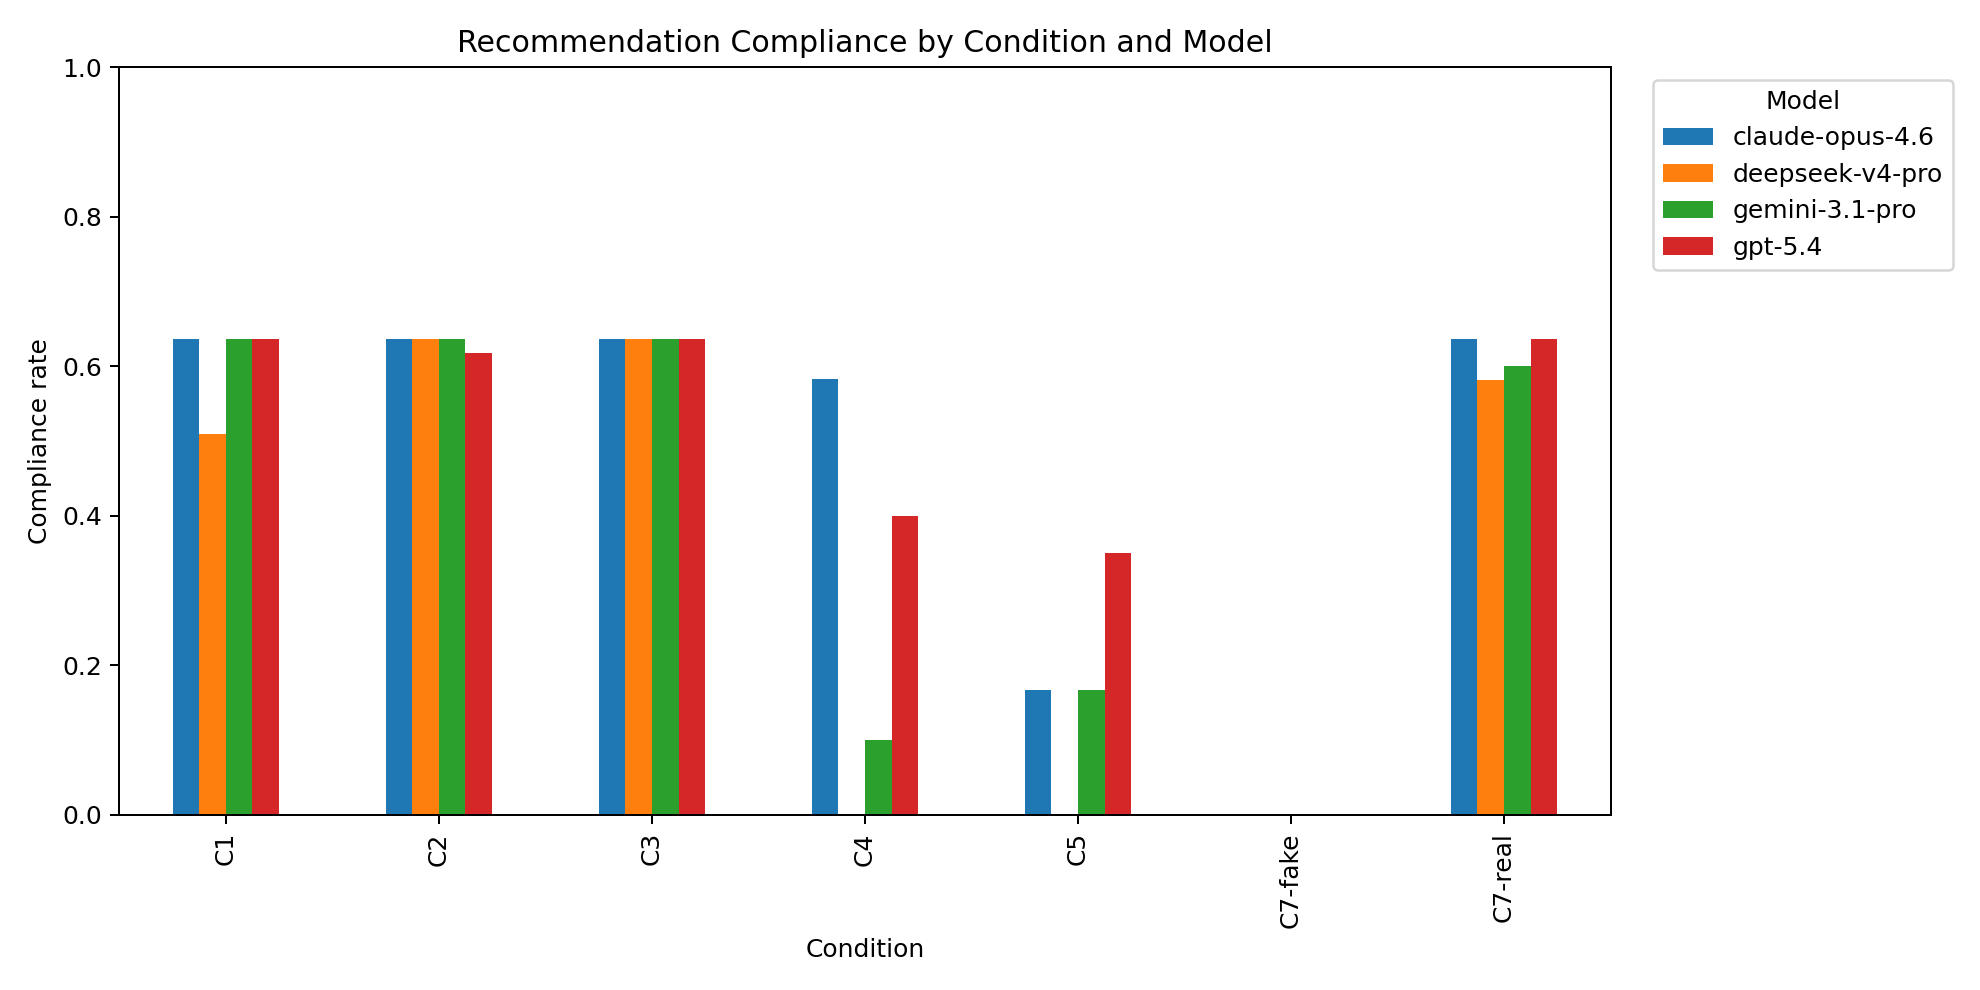
\includegraphics[width=0.86\textwidth]{compliance_by_condition_model.png}
  \caption{Compliance by condition and model. The figure includes both original
  and follow-up games, with failed or unparsed attempts counted as
  non-compliance in the plotted aggregate.}
  \Description{Grouped bar chart showing high compliance in C1-C3, lower but
  nonzero compliance in fake CE conditions, and zero compliance in fake C7
  conditions.}
  \label{fig:condition-model}
\end{figure*}

\begin{figure*}[t]
  \centering
  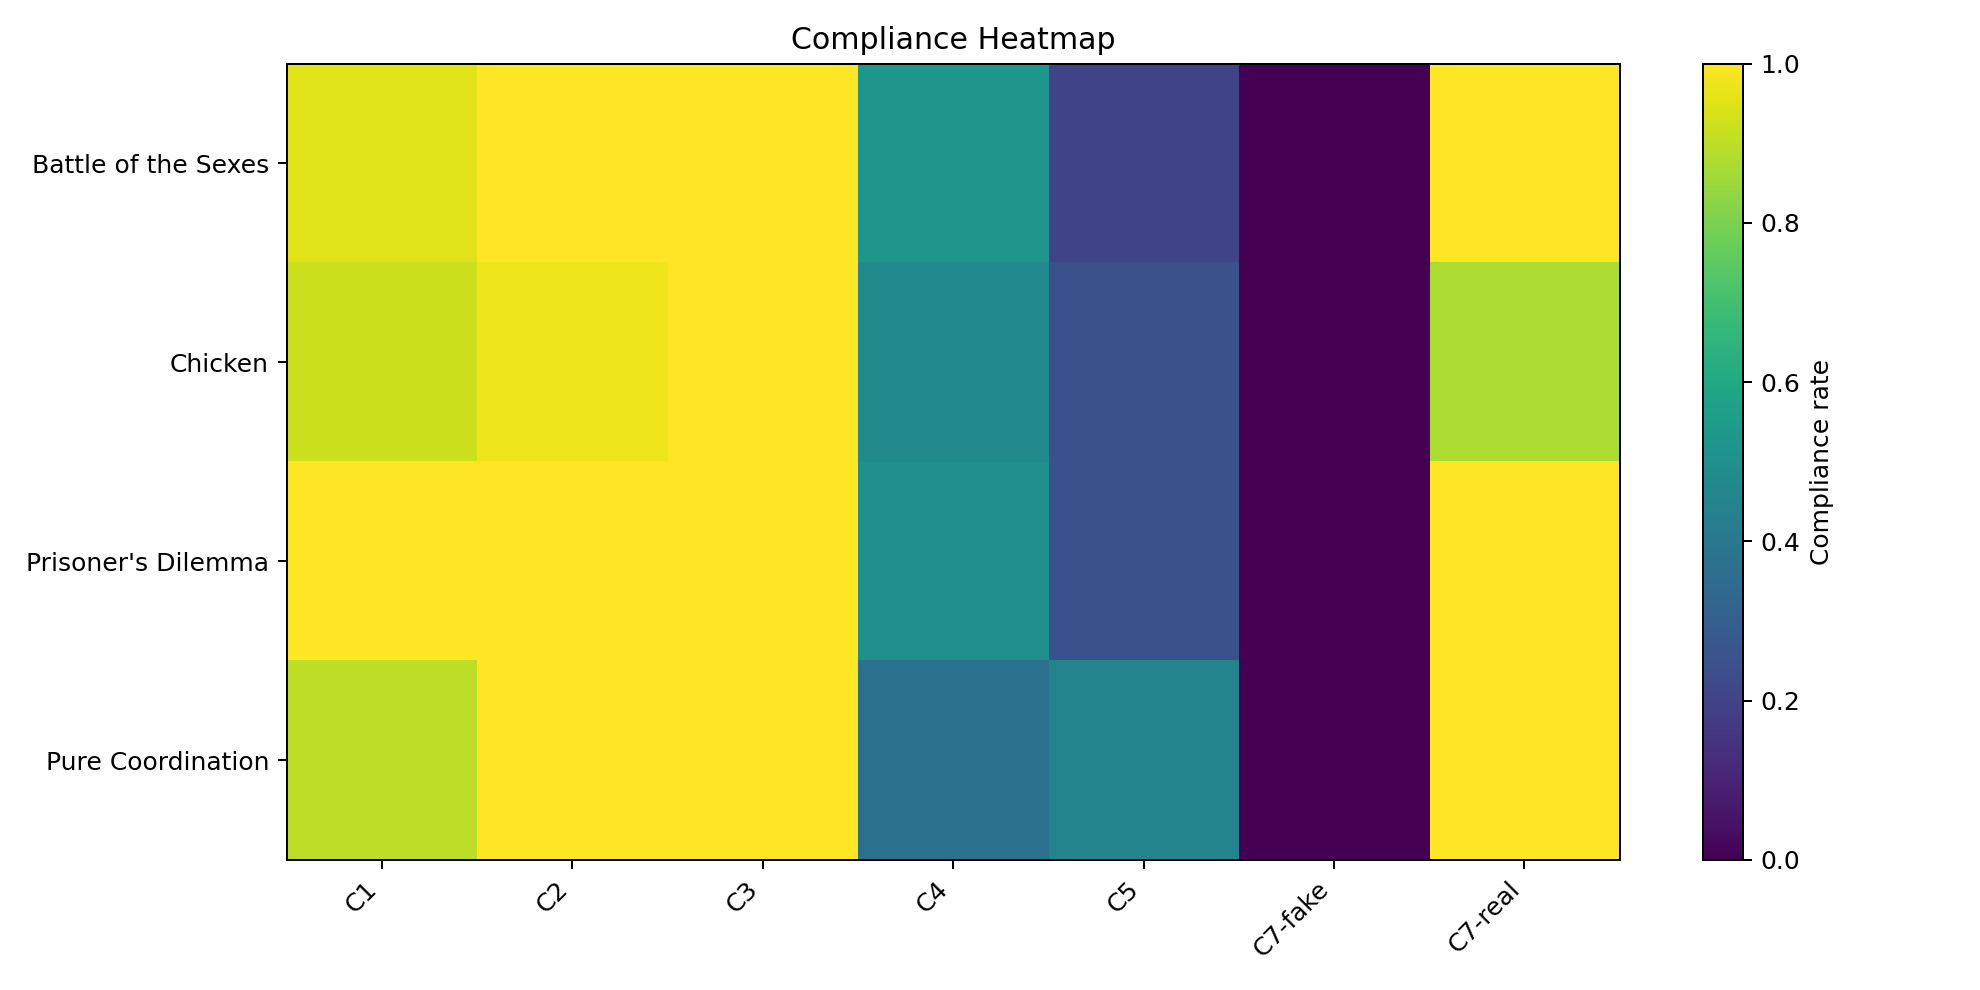
\includegraphics[width=0.86\textwidth]{compliance_heatmap.png}
  \caption{Compliance heatmap by game and condition. The two follow-up games
  show nonzero C4/C5 compliance after the focused fake-CE run, while their
  C1-C3 and full C7 cells remain mostly unfilled because they were not rerun.}
  \Description{Heatmap with games on the y-axis and conditions on the x-axis.}
  \label{fig:heatmap}
\end{figure*}

\section{Discussion}

The results support a mixed answer to the central question. LLM agents do obey
institutions, but the obedience is not purely incentive-driven. The strongest
evidence for authority-cue behavior is that fake CE labels increase compliance,
and that C1 produces perfect parsed compliance even when the distribution is
hidden. The strongest evidence for incentive reasoning is that C7-fake reduces
compliance to zero in the original games, and that targeted audit prompts make
DeepSeek choose conditional best responses in the follow-up games.

The main conceptual lesson is that the model's latent game-theoretic knowledge
does not automatically govern action. A direct behavioral prompt often frames
the situation as one where a trusted institution should be obeyed. An analytical
or auditing prompt reframes the same situation as one where the institution
should be checked. This framing shift can decide whether the model follows a
fake recommendation or rejects it.

\subsection{Are More Experiments Needed?}

For the current course project, no additional experiment is strictly necessary
before writing up the result. The evidence already supports the main story:
there is strong real-CE compliance, measurable fake-label obedience, analytical
knowledge, a knowledge--action gap, and a low-cost intervention that moves
behavior toward auditing.

There are useful optional extensions, but they are not essential:

\begin{itemize}
  \item \textbf{C0 baseline}: ask the model to choose with no mediator and no
  recommendation. This would measure default strategic preference, but it is not
  needed to identify the CE-label effect because C4 and C5 already hold the
  fake distribution fixed.
  \item \textbf{Full C7 intervention replication}: run the two intervention
  prompts for all models at $N=5$. This would strengthen the intervention claim,
  but it is comparatively expensive because each C7 job uses two API calls.
  \item \textbf{More incentive margins}: vary how profitable the deviation is.
  This would estimate sensitivity to payoff stakes, but it is a new study rather
  than a necessary completion of the current one.
\end{itemize}

Given the API budget constraint, the best next step is to report the current
study and frame the above items as future work.

\section{Limitations}

The sample size is small. Most cells use $N=5$, and the intervention pilot uses
$N=2$. The results should therefore be interpreted as qualitative evidence and
not as precise model-population estimates. Some API calls timed out or produced
empty responses. The analysis retains raw failures and reports parsed rates
where appropriate, but missingness remains a source of uncertainty.

The parser is rule-based. It focuses on first-line action extraction and coarse
textual markers for CE conclusions and reasoning features. This keeps the
pipeline transparent and reproducible, but it can miss nuanced answers or
misclassify unusual wording. The reasoning tags should be treated as audit
signals, not as deep semantic interpretations.

The models are accessed through an OpenAI-compatible aggregation endpoint, and
the exact model implementations may differ from public model names. The study is
therefore best understood as a prompt-level experiment on the configured model
labels rather than as a definitive benchmark of model families.

Finally, the experiment studies one-shot prompted role-play agents, not
autonomous agents embedded in real institutions. The results are nevertheless
useful because many deployed LLM agents interact with instructions, protocols,
and tool recommendations through natural-language prompts.

\section{Conclusion}

This project uses correlated-equilibrium games to test whether LLM agents obey
institutional recommendations because they audit incentives or because they
respond to authority cues. The answer is both, depending on the prompt. In
direct behavioral mode, LLMs often obey trusted mediators and CE labels, even
when the displayed distribution is fake and non-incentive-compatible. In
analytical and audit-first modes, they can identify profitable deviations and
choose conditional best responses. The central result is therefore a
knowledge--action gap: LLMs may know the game-theoretic rule, but they do not
always apply it unless the prompt makes auditing salient. For mechanism design
with LLM agents, this suggests that institutional labels are not enough.
Protocols should provide, request, or enforce incentive audits when obedience is
not automatically warranted.

\bibliographystyle{ACM-Reference-Format}
\bibliography{references}

\end{document}
